\documentclass[ 12pt ]{article}
\usepackage{amsmath, amsthm, amssymb, enumitem, graphicx, listings, mathrsfs}
\usepackage[margin=0.5in]{geometry}
\graphicspath{ ./ }

\begin{document}

\noindent Landon Fox \\
\noindent Math 485 \\
\noindent November 25, 2020 \\
\noindent \textbf{Collaborated with Logan Leavitt}

\begin{center}
	\Large Homework 9
\end{center}

\begin{enumerate}
	% problem 1
	\item[\textbf{1.}]
		\begin{enumerate}
			\item[\textbf{i.}] Prove that the distance function $d(u, v)$ satisfies the triangle-inequality.
			\item[\textbf{ii.}] Show that diam$(G) \leq 2$rad$(G)$ for every graph $G$.
			\item[\textbf{iii.}] For all $r, d \in \mathbb{N}$ with $r \leq d \leq 2r$, construct a simple graph with the radius $r$ and diameter $d$.
		\end{enumerate}

		\begin{proof}
			\begin{enumerate}
				\item[\textbf{i.}] Suppose $G$ is a graph with $u, v, w \in V(G)$. Consider the case where $w$ belongs to the shortest $uv$-path. Then it follows that $$d(u, v) =
					d(u, w) + d(w, v).$$ Now, suppose $w$ does not belong to the shortest $uv$-path; in other words, all $uv$-paths that include $w$ are not minimal. Therefore,
					$$d(u, v) < d(u, w) + d(w, v).$$

				\item[\textbf{ii.}] Again, suppose $G$ is a graph with $u, v, w \in V(G)$. Further, suppose diam$(G) = d(u, v)$ and rad$(G) = \epsilon(w)$. By the result of \textbf{1i},
					we know that $$d(u, v) \leq d(u, w) + d(w, v).$$ Then by the maximality of $\epsilon(w)$, it follows that $$\mathrm{diam}(G) = d(u, v) \leq d(u, w) + d(w, v) \leq
					\epsilon(w) + \epsilon(w) = 2\mathrm{rad}(G).$$

				\item[\textbf{iii.}] Let $G$ be a graph defined as
					\begin{center}
						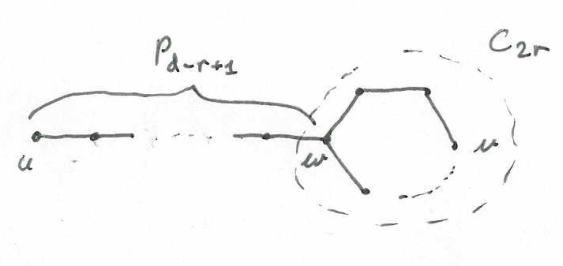
\includegraphics{Capture}
					\end{center}
					Clearly, diam$(G) = d(u, v) = d$. In regard to the radius, I claim that $w$ must be within the
					center of $G$. Observe that any vertex in $C_{2r}$ will have an eccentricity of at least $r$ and any vertex in $P_{d - r + 1}$, other than $w$, will have
					eccentricity greater than $r$. Therefore, $w$ belongs to the center of $G$ since $\epsilon(w) = r$ and so rad$(G) = r$.
			\end{enumerate}
		\end{proof}


	% problem 2
	\item[\textbf{2.}]
		\begin{enumerate}
			\item[\textbf{i.}] Let $n \geq 2$ and $d_1, d_2, \hdots, d_n \in \mathbb{N}$. Prove that there exists a tree with vertex degrees $d_i$ if and only if $\sum_{i \in [n]}d_i
				= 2n - 2$.
			\item[\textbf{ii.}] Given $d_1, d_2, \hdots, d_n \in \mathbb{N}$ such that $\sum_{i \in [n]} d_i = 2n - 2$, show that there are $$(n-2)!\prod_{i \in [n]}\frac{1}{ (d_i -
				1)!}$$ trees on $[n]$ such that vertex $i$ has degree $d_i$ for each $i \in [n]$.
			\item[\textbf{iii.}] Let $T$ and $T'$ be two trees on the same vertex set such that $d_T(v) = d_{T'}(v)$ for every $v$ in the vertex set. Show that $T'$ can be obtained
				from $T$ by a sequence of 2-switches such that every graph along the way is also a tree.
		\end{enumerate}

		\begin{proof}
			\begin{enumerate}
				\item[\textbf{i.}] Suppose $T$ is an $n$-vertex tree with $n \geq 2$ and a degree sequence $d_1, d_2, \hdots, d_n \in \mathbb{N}$. Then it follows that $|E(T)| = n - 1$
					and so $$\sum_{i \in [n]} d_i = 2(n - 1)$$ by the Handshaking Lemma. \\ \\
					Conversely, let $n \geq 2$, $d_1, d_2, \hdots, d_n \in \mathbb{N}$, and $\sum_{i \in [n]} d_i = 2n - 2$. Observe that there exists a $d_j$ such that $d_j = 1$;
					otherwise, $d_i \geq 2$ for all $i \in [n]$ which implies that $$\sum_{i \in [n]} d_i \geq 2n.$$ Similarly, we can conclude that there is a $d_k \geq 2$ when $n >2$.
					\\ \\
					Now, as a base case, $n = 2$, it must hold that $d_1 = d_2 = 1$ which is clearly realizable by a tree. For the inductive step, suppose that exists a tree for any 
					degree sequence $\{ d_i \in \mathbb{N} \}_{i \in [n]}$ for a particular $n \geq 2$ such that $\sum_{i \in [n]} d_i = 2n - 2$. Consider a degree sequence $\{ d_i \in 
					\mathbb{N} \}_{i \in [n+1]}$ of length $n + 1$. As previously shown, there must exist $j \neq k \in [n + 1]$ such that $d_j = 1$ and $d_k > 1$. Hence, $$d_1, \hdots,
					d_{j-1}, d_{j+1}, \hdots, d_k - 1, \hdots, d_{n+1}$$ is realizable by a tree $T$ and so is our degree sequence of length $n+1$ by adding a leaf to the vertex $k$ of
					$T$.

				\item[\textbf{ii.}] Provided a degree sequence $d_1, d_2, \hdots, d_n \in \mathbb{N}$ such that $\sum_{i \in [n]} d_i = 2n - 2$, we know that it is realizable by a tree
					via \textbf{2i}. Using a Pr$\ddot{\mathrm{u}}$fer code, we can uniquely encode our degree sequence. Since there must be $n - 1$ edges in our tree and the last in our
					Pr$\ddot{\mathrm{u}}$fer code is reserved for the root of the tree, there are $n - 2$ placements for parents. Additionally, there is no variation is the placement of
					the children. Furthermore, there are $d_i - 1$ repeats for every parent $i \in [n]$ which illustrates that there are $$(n-2)!\prod_{i \in [n]}\frac{1}{ (d_i - 1)!}$$
					possible trees.

				\item[\textbf{iii.}] Suppose $T$ and $T'$ are two trees with $V(T) = V(T') = [n]$ such that $d_T(v) = d_{T'}(v)$ for all $v \in [n]$. As a base case, let $n \leq 3$.
					For any tree to have $n$ vertices, it must be isomorphic $P_n$ and so $T = T'$ which vacuously holds. In regard to the inductive step suppose for $n-1 \geq 3$, $T$
					can always be transformed to $T'$ by a series of 2-switches such that it always remains to be a tree. Now consider a vertex set of size $n$ and a leaf $u$ in $T$ with
					a parent $v$. If $v$ is the parent of $u$ in $T'$ then we can remove $u$ from both trees and apply the inductive hypothesis since $u$ must also be a leaf in $T'$.
					Otherwise, let $w$ be the parent of $u$ in $T'$. Due to the fact that trees are connected by definition, it must hold that $d(w) \geq 2$. Let $x, y$ denote two
					vertices adjacent to $w$ in $T$. Then it follows that $v$ cannot be adjacent to both $x$ and $y$. Now perform a 2-switch with the edges $uv$ and $wx$ (or $wy$ if
					$v$ is adjacent to $x$) to obtain $uw$ and $vx$ ($vy$, respectively) ensuring that $T$ has no cycles. Hence, the inductive hypothesis can be applied after removing
					$u$ from both $T$ and $T'$ proving the claim.
			\end{enumerate}
		\end{proof}


	% problem 3
	\item[\textbf{3.}] Show that if $T$ is a tree with $k$ leaves, the $T$ is the union of $\left \lceil \frac{k}{2} \right \rceil$ pairwise intersecting paths.

		\begin{proof}
			Suppose $T$ is a tree with $k$ leaves. Let the leaves be denoted $w_1, \hdots, w_k$. Further, suppose we pair the leaves arbitrarily, repeating a vertex if $k$ is odd
			to create $\left \lceil \frac{k}{2} \right \rceil$ paths denoted by $P_{w_i, w_j}$. Consider the paths $P_{w_i, w_j}$ and $P_{w_k, w_\ell}$ with no intersection. I claim that
			$P_{w_i, w_\ell}$ and $P_{w_k, w_j}$ have a nonempty intersection and their union strictly increases the coverage of $T$ so that all existing intersecting paths are not
			altered. Observe that there can only exist one path from $P_{w_i, w_j}$ to $P_{w_k, w_\ell}$, represented as $P_{x, y}$ with $x \in P_{w_i, w_j}$ and $y \in P_{w_k, w_\ell}$,
			otherwise cycles would exist; furthermore, both $P_{w_i, w_\ell}$ and $P_{w_k, w_j}$ must use $P_{x, y}$ and so they must have a nonempty intersection. Additionally,
			it follows that $$P_{w_i, w_j} \cup P_{w_k, w_\ell} = P_{w_i, x} \cup P_{x, w_j} \cup P_{w_k, y} \cup P_{y, w_\ell} \subset P_{w_i, x} \cup P_{x, w_j} \cup P_{w_k, y}
			\cup P_{y, w_\ell} \cup P_{x, y} = P_{w_i, w_\ell} \cup P_{w_k, w_j}.$$ Therefore, this process can be repeated until all paths are no longer disjoint; however, it remains
			to be shown that $T$ will be covered when all paths are pairwise intersecting. \\ \\
			Suppose $T$ is not covered by a union of the $\left \lceil \frac{k}{2} \right \rceil$ paths; in other words, the union of the paths does not include an edge of $T$.
			Since every edge of a tree is a cut edge, it must be the case that the union of the paths are disconnected, implying that there exists disjoint paths. Thus, by
			contraposition we can conclude that $T$ is covered when there are no disjoint paths.
		\end{proof}


	% problem 4
	\item[\textbf{4.}]
		\begin{enumerate}
			\item[\textbf{i.}] Given a connected weighted graph $G$, start from any vertex and iteratively add the cheapest edge from the vertex already reached to a vertex not yet
				reached. Finish when all vertices are reached. Show that the algorithm produces a minimum spanning tree.
			\item[\textbf{ii.}] Let $G$ be a weighted graph with distinct weights on its edges. Show that $G$ has a unique minimum spanning tree.
		\end{enumerate}

		\begin{proof}
			\begin{enumerate}
				\item[\textbf{i.}] Suppose $G$ is a connected weighted graph and apply Prim's Algorithm to it to obtain $T$. Provided that $G$ is connected, its clear that all
					newly added edges will strictly decrease the number of components implying that $T$ is connected. Additionally, if a cycle did exist in $T$ then it would illustrate
					that the algorithm added an edge to a vertex already reached. Therefore, $T$ is a spanning tree of $G$. \\ \\
					Suppose by contradiction that $T' \neq T$ is a minimum spanning tree of $G$. Let $e$ be the first edge chosen for $T$ such that $e \notin T'$. Then we know that
					there exists an $e' \notin T$ but $e' \in T'$ such that $T' + e - e'$ is a spanning tree. Consider the case where $e'$ was unreachable when $e$ was chosen. Further,
					if $e'$ is the minimal weight of one of the vertices it is incident to, then the algorithm must choose $e$ once it reaches one of the vertices because it locally chooses
					the minimal weight. If it is not the minimal weight to either of its incident vertices then it must contradict the minimality of $T'$. Otherwise, if $e'$ was locally
					available to $T$ at the time of choosing $e$, then $w(e) \leq w(e')$. Thus, $w(T' + e - e') \leq w(T')$ and this process can be done repeatedly until all edges
					align to $T$ and so $T$ is a minimum spanning tree.

				\item[\textbf{ii.}] Let $G$ be a weighted graph with distinct edge weights. Suppose by contradiction that $G$ has two distinct minimum spanning trees $T$ and $T'$.
					For the trees to be distinct, there must exist an edge $e \in T$ such that $e \notin T'$. Then we know that we can choose an $e' \in T' - T$ such
					that $T' + e - e'$ is a spanning tree of $G$. Observe that $w(e) \neq w(e')$ because $e \neq e'$. Without loss of generality, suppose $w(e) < w(e')$. However,
					$w(T' + e - e') < w(T')$ which is a contradiction.
			\end{enumerate}
		\end{proof}


	% problem 5
	\item[\textbf{5.}]
		\begin{enumerate}
			\item[\textbf{i.}] Prove that the number of spanning trees of $K_{2, n}$ is $n2^{n-1}$.
			\item[\textbf{ii.}] Find the number of ordered full binary rooted trees with $n+1$ leaves.
		\end{enumerate}

		\begin{proof}
			\begin{enumerate}
				\item[\textbf{i.}] Consider the graph $K[X, Y]$ where $|X| = 2$ and $|Y| = n$. To create a spanning tree, let us first choose one vertex in $Y$ to be adjacent to
					both vertices in $X$ to ensure our tree is connected. With the remaining $n-1$ vertices in $Y$, draw a single edge between a vertex in $Y$ to an arbitrary vertex
					in $X$. Thus, the number of spanning trees of $K_{2, n}$ is $n2^{n-1}$.

				\item[\textbf{ii.}] Let $C_n$ denote the number of ordered full binary rooted trees with $n+1$ leaves. Observe that for every vertex in our tree, we have to assign
					leaves to the left and right children, dictating the form of the tree. Since we must ensure that at least one leaf is designated to both children, let us designate
					one leaf to always take the left child unless that right child has no leaves. Then it follows that $$C_n = C_0 C_{n-1} + C_1 C_{n-2} + \hdots + C_{n-1} C_0 = 
					\sum_{k = 0}^{n-1} C_k C_{n - k - 1}.$$ Also, notice that $C_0 = 1$ and so $C_n$ is the Catalan Numbers shifted by one index!
			\end{enumerate}
		\end{proof}


	% problem 6
	\item[\textbf{6.}] Prove that if $T_1, T_2, \hdots, T_k$ are pairwise intersecting subtrees of a tree $T$, then $T$ has a vertex common to all $T_i$.

		\begin{proof}
			Suppose $T_1, T_2, \hdots, T_k$ are pairwise intersecting subtrees of a tree $T$. As a base case, $k = 2$, this clearly holds. For the inductive step, suppose
			for $k-1 \geq 2$ that $T_1, T_2, \hdots, T_{k-1}$ all have one vertex in common, denoted $u$. Consider an additional subtree $T_k$ of $T$ with pairwise intersections with
			all $k-1$ other subtrees. Suppose by contradiction that $u$ does not belong to $T_k$. Provided the vertices within the pairwise intersections, $u_1, u_2, \hdots, u_r$ where
			$2 \leq r \leq k$, observe that the paths $P_{u, u_1}$ in subtree $T_1$, $P_{u_1, u_2}$ in subtree $T_k$, and $P_{u_2, u}$ in subtree $T_2$ create a cycle which is a
			contradiction.
		\end{proof}
\end{enumerate}

\end{document}
